\documentclass{article}

\usepackage{graphicx}
\usepackage{tikz}
\usepackage{tikzsymbols}
\usetikzlibrary{calc,patterns,shapes.geometric}
\pagestyle{empty}
\usepackage[margin=0pt]{geometry}
\geometry{papersize={14in,12in}}

\def\centerarc[#1](#2)(#3:#4:#5){\draw[#1] ($(#2)+({#5*cos(#3)},{#5*sin(#3)})$) arc (#3:#4:#5);}

\begin{document}
	\begin{figure}
		\centering
		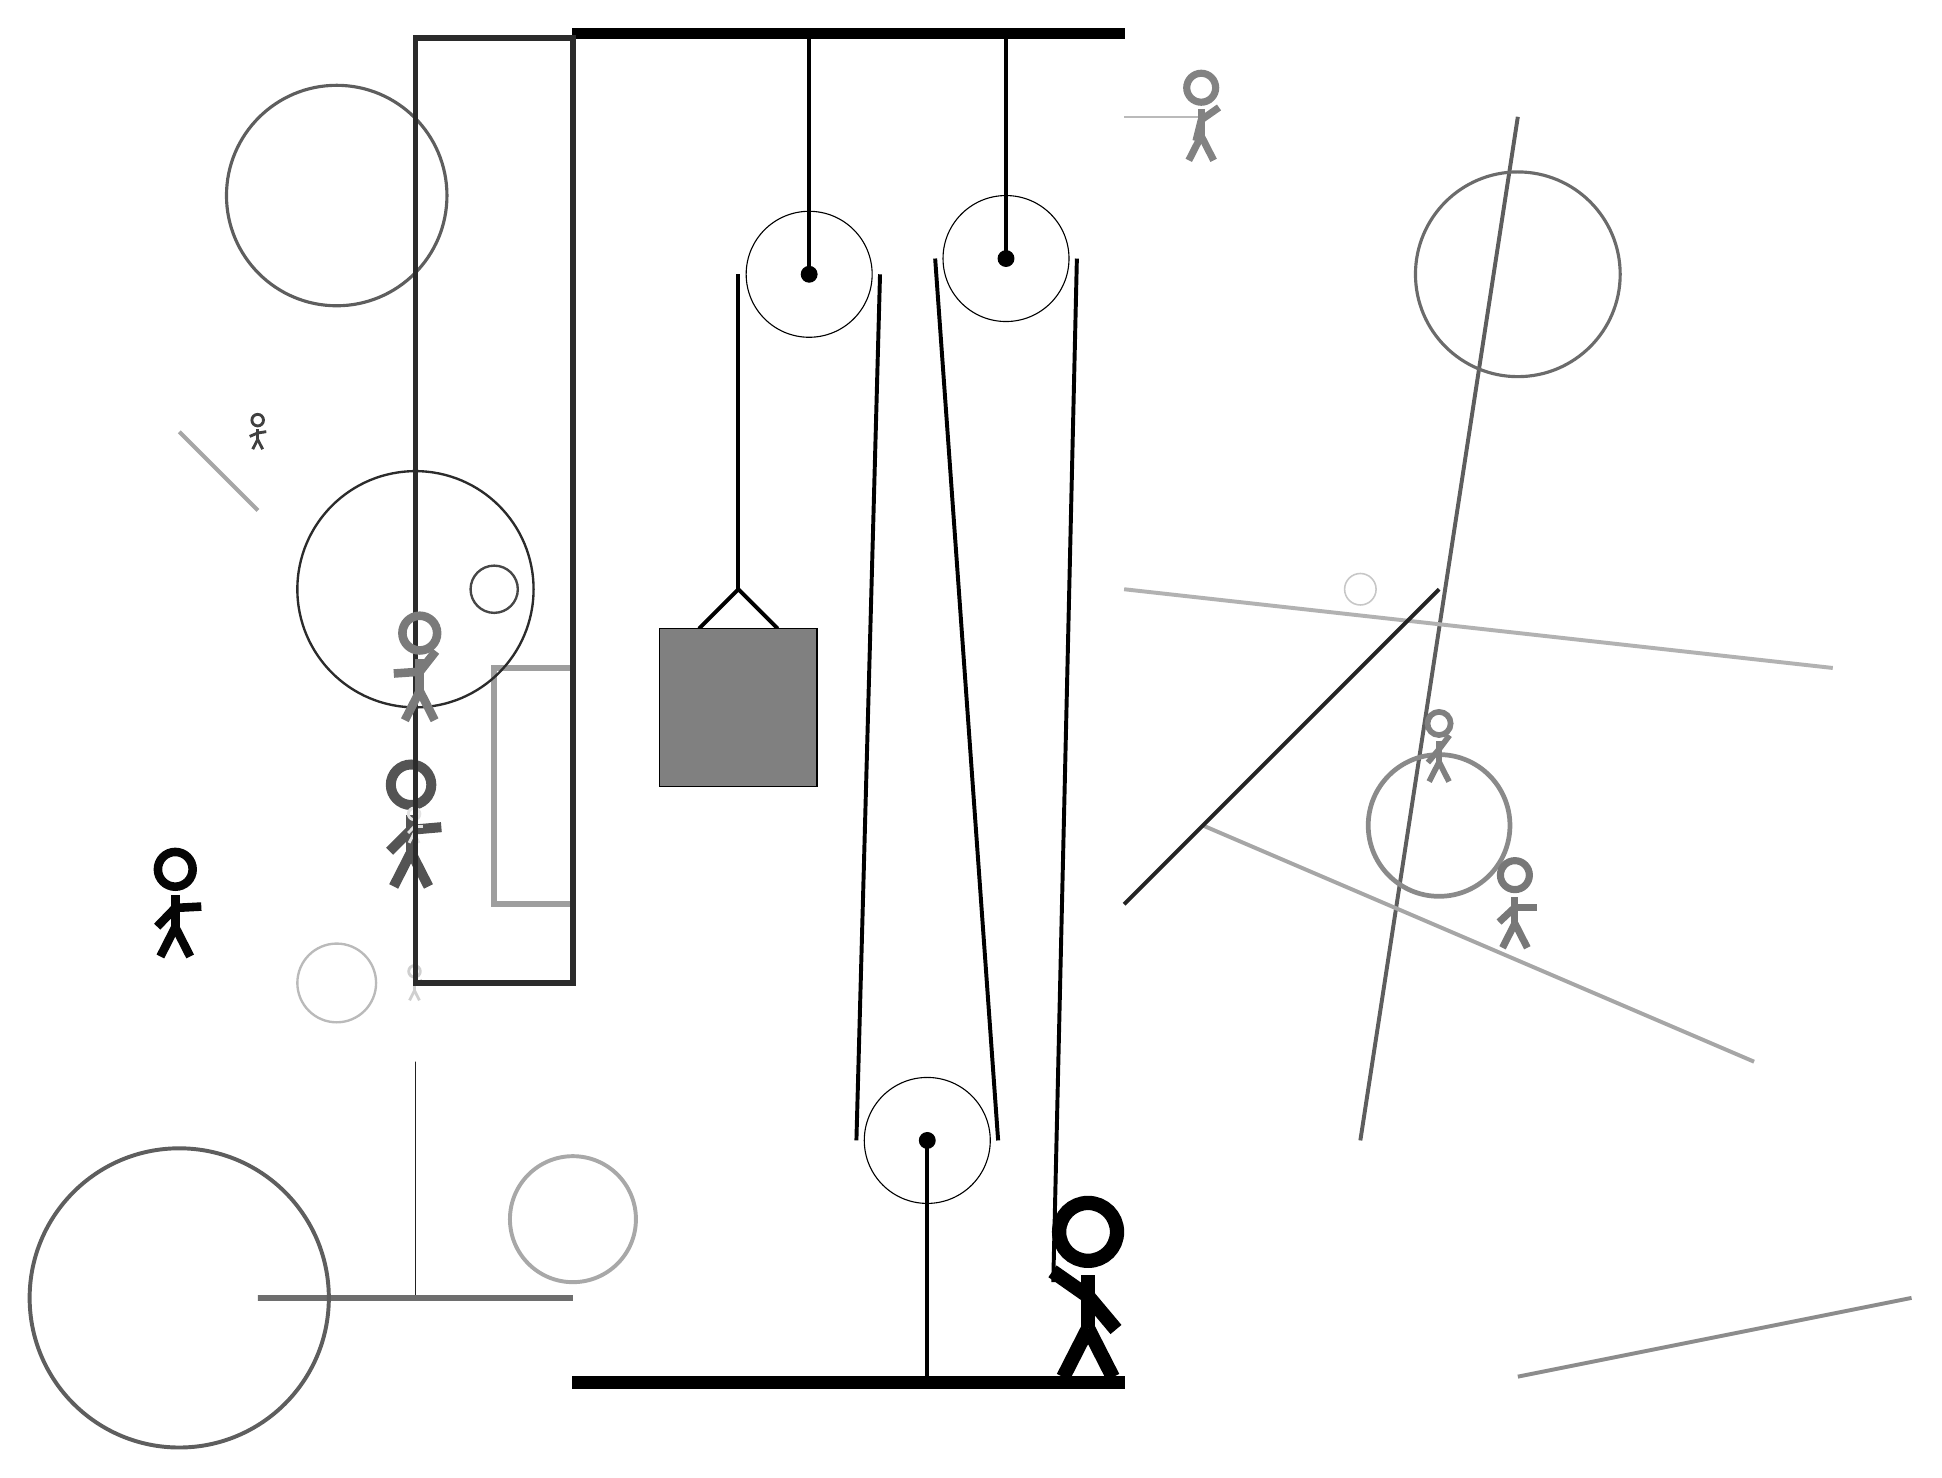
\begin{tikzpicture}
			%%%%% START %%%%%
			
			\draw[fill=black] (-2, 14) rectangle (5, 14.125);
			
			\draw (1, 11) circle (0.8);
			\draw[fill=black] (1, 11) circle (0.1);
			\draw[line width=0.5mm]  (1, 14) -- (1, 11);
			
			\draw[fill=white](2.5, 0) circle (0.8);
			\draw[fill=black] (2.5, 0) circle (0.1);
			\draw[line width=0.5mm]  (2.5, -3) -- (2.5, 0);
			
			\draw[line width=0.7mm, color=black!38] (-3, 3) rectangle (-2, 6);
			
			\draw[line width=0.3mm, color=black!27] (6, 13) rectangle (5, 13);
			\draw [line width=0.4mm, color=black!63](-5, 12) circle (1.4);
			\node[line width=0.4mm, color=black!67] at (-4, 4) {\Strichmaxerl[7][45][5]};
			
			\draw[line width=0.5mm, color=black!35](-6, 8) -- (-7, 9);
			\node[line width=0.5mm, color=black!98] at (-7, 3) {\Strichmaxerl[6][46][3]};
			\node[line width=0.2mm, color=black!19] at (-4, 2) {\Strichmaxerl[2][90][27]};
			\draw [line width=0.3mm, color=black!27](-5, 2) circle (0.5);
			\draw[line width=0.5mm, color=black!63](8, 0) -- (10, 13);
			\draw [line width=0.2mm, color=black!22](8, 7) circle (0.2);
			\node[line width=0.7mm, color=black!11] at (-4, 4) {\Strichmaxerl[2][47][0]};
			
			\draw [line width=0.4mm, color=black!58](10, 11) circle (1.3);
			\draw[line width=0.7mm, color=black!83] (-4, 2) rectangle (-2, 14);
			
			\draw [line width=0.6mm, color=black!46](9, 4) circle (0.9);
			\node[line width=0.5mm, color=black!50] at (9, 5) {\Strichmaxerl[4][50][53]};
			\draw [line width=0.3mm, color=black!83](-4, 7) circle (1.5);
			\draw[line width=0.5mm, color=black!35](6, 4) -- (13, 1);
			
			\draw[line width=0.2mm, color=black!87] (-4, 1) rectangle (-4, -2);
			\draw[line width=0.5mm, color=black!30](5, 7) -- (14, 6);
			\draw[line width=0.5mm, color=black!45](10, -3) -- (15, -2);
			\node[line width=0.5mm, color=black!49] at (6, 13) {\Strichmaxerl[5][76][35]};
			
			\draw[line width=0.7mm, color=black!57] (-2, -2) rectangle (-6, -2);
			\draw [line width=0.5mm, color=black!63](-7, -2) circle (1.9);
			\node[line width=0.2mm, color=black!52] at (-4, 6) {\Strichmaxerl[6][4][52]};
			\node[line width=0.4mm, color=black!53] at (10, 3) {\Strichmaxerl[5][43][0]};
			\draw [line width=0.5mm, color=black!34](-2, -1) circle (0.8);
			\draw [line width=0.3mm, color=black!72](-3, 7) circle (0.3);
			\node[line width=0.5mm, color=black!75] at (-6, 9) {\Strichmaxerl[2][23][9]};
			
			\draw[line width=0.5mm, color=black!86](9, 7) -- (5, 3);
			
			\draw[fill=white](3.5, 11.2) circle (0.8);
			\draw[fill=black] (3.5, 11.2) circle (0.1);
			\draw[line width=0.5mm] (3.5, 14) -- (3.5, 11.2);
			
			\draw[line width=0.5mm] (-0.4, 6.5) -- (0.1, 7.0) -- (0.6, 6.5);
			\draw[fill=black!50] (-0.9, 6.5) rectangle (1.1, 4.5);
			
			\draw[line width=0.5mm] (0.1, 11) -- (0.1, 7.0);
			\centerarc[line width=0.5mm](1, 11)(0:180:0.9);
			\draw[line width=0.5mm](1.9, 11) -- (1.6, 0);
			\centerarc[line width=0.5mm](2.5, 0)(180:360:0.9);
			\draw[line width=0.5mm](3.4, 0) -- (2.6, 11.2);
			\centerarc[line width=0.5mm](3.5, 11.2)(0:180:0.9);
			\draw[line width=0.5mm](4.4, 11.2) -- (4.1, -1.8);
			
			\node at (4.5, -1.9) {\Strichmaxerl[10][-35][-50]};
			
			\draw[fill=black] (-2, -3) rectangle (5, -3.15);
			
			%%%%% END %%%%%
		\end{tikzpicture}
	\end{figure}	
\end{document}